\documentclass[tikz,border=12pt]{standalone}
\usepackage[T1]{fontenc}
\usepackage{mathpazo}
\usepackage{amsmath,amssymb}
\usetikzlibrary{arrows.meta, positioning, calc, fit}

\definecolor{stblue}{HTML}{7B97AD}
\definecolor{rwgold}{HTML}{B8995E}
\definecolor{sage}{HTML}{7A9A7E}
\definecolor{dkbrown}{HTML}{3D3530}
\definecolor{wmgray}{HTML}{7B7067}
\definecolor{cream}{HTML}{F9F6F0}
\definecolor{border}{HTML}{D4C9B8}
\definecolor{terracotta}{HTML}{C47A6A}
\definecolor{lavender}{HTML}{907EA0}

\begin{document}
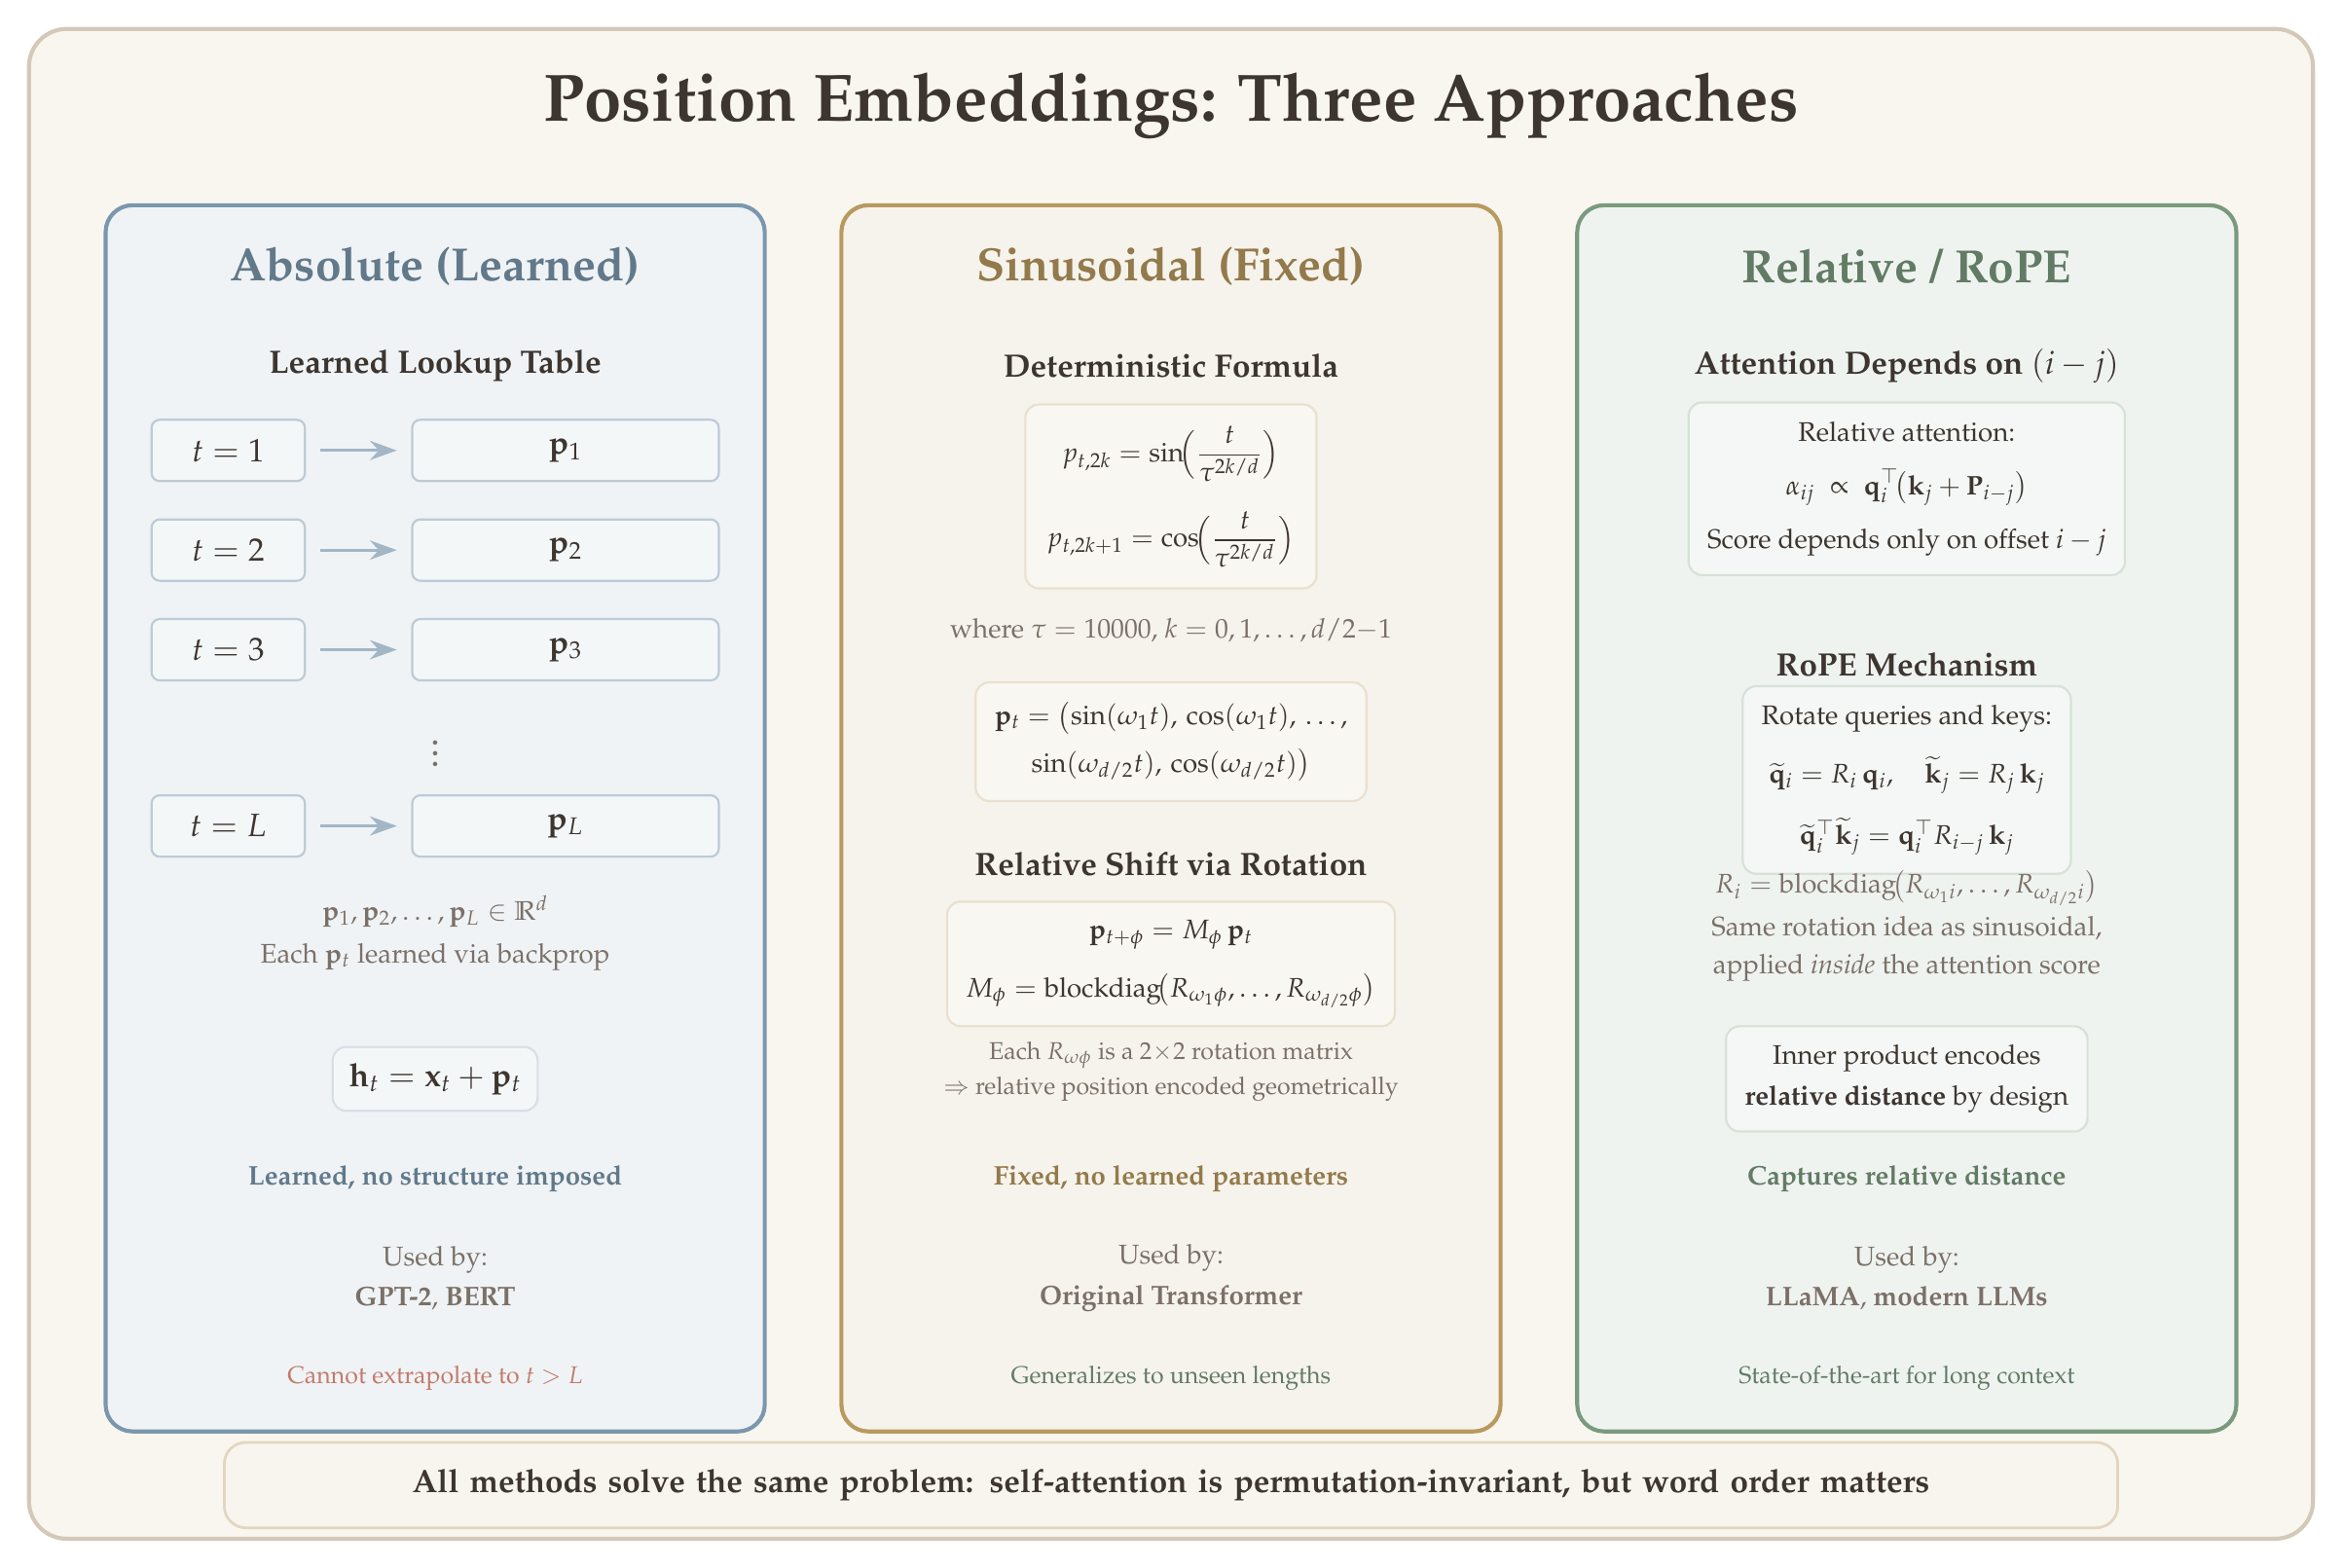
\begin{tikzpicture}[
  >={Stealth[length=3.5mm, width=2.5mm]},
]

% ── Global dimensions ──
\pgfmathsetmacro{\colw}{8.6}   % column width
\pgfmathsetmacro{\colh}{13.5}  % column inner height
\pgfmathsetmacro{\gap}{1.0}    % gap between columns
\pgfmathsetmacro{\totalw}{3*\colw + 2*\gap + 2} % total width with margins

% Background
\fill[cream, rounded corners=14pt] (-1,-2.2) rectangle (\totalw-1, 17.5);
\draw[border, rounded corners=14pt, line width=1.5pt] (-1,-2.2) rectangle (\totalw-1, 17.5);

% Title
\node[font=\Huge\bfseries, text=dkbrown] at ({(\totalw-2)/2}, 16.5)
  {Position Embeddings: Three Approaches};

% ============================================================
% COLUMN 1: Absolute (Learned) — stblue
% ============================================================
\pgfmathsetmacro{\coneL}{0}
\pgfmathsetmacro{\coneR}{\coneL + \colw}
\pgfmathsetmacro{\coneMid}{(\coneL + \coneR)/2}

% Column box
\fill[stblue!12, rounded corners=10pt] (\coneL, -0.8) rectangle (\coneR, 15.2);
\draw[stblue, rounded corners=10pt, line width=1.5pt] (\coneL, -0.8) rectangle (\coneR, 15.2);

% Column title
\node[font=\LARGE\bfseries, text=stblue!80!black] at (\coneMid, 14.4)
  {Absolute (Learned)};

% Lookup table illustration
\node[font=\large\bfseries, text=dkbrown] at (\coneMid, 13.1)
  {Learned Lookup Table};

% Table grid: position -> vector
\foreach \i/\lab in {1/1, 2/2, 3/3} {
  \pgfmathsetmacro{\yy}{12.0 - (\i-1)*1.3}
  % Position cell
  \fill[stblue!8, rounded corners=3pt]
    (\coneL+0.6, \yy-0.4) rectangle (\coneL+2.6, \yy+0.4);
  \draw[stblue!50, rounded corners=3pt, line width=0.8pt]
    (\coneL+0.6, \yy-0.4) rectangle (\coneL+2.6, \yy+0.4);
  \node[font=\large, text=dkbrown] at (\coneL+1.6, \yy)
    {$t = \lab$};
  % Arrow
  \draw[->, line width=1.2pt, stblue!70] (\coneL+2.8, \yy) -- (\coneL+3.8, \yy);
  % Vector cell
  \fill[stblue!8, rounded corners=3pt]
    (\coneL+4.0, \yy-0.4) rectangle (\coneR-0.6, \yy+0.4);
  \draw[stblue!50, rounded corners=3pt, line width=0.8pt]
    (\coneL+4.0, \yy-0.4) rectangle (\coneR-0.6, \yy+0.4);
  \node[font=\large, text=dkbrown] at ({(\coneL+4.0+\coneR-0.6)/2}, \yy)
    {$\mathbf{p}_{\lab}$};
}

% Dots
\node[font=\Large, text=wmgray] at (\coneMid, 8.15) {$\vdots$};

% Last row: position L
\pgfmathsetmacro{\ylast}{7.1}
\fill[stblue!8, rounded corners=3pt]
  (\coneL+0.6, \ylast-0.4) rectangle (\coneL+2.6, \ylast+0.4);
\draw[stblue!50, rounded corners=3pt, line width=0.8pt]
  (\coneL+0.6, \ylast-0.4) rectangle (\coneL+2.6, \ylast+0.4);
\node[font=\large, text=dkbrown] at (\coneL+1.6, \ylast)
  {$t = L$};
\draw[->, line width=1.2pt, stblue!70] (\coneL+2.8, \ylast) -- (\coneL+3.8, \ylast);
\fill[stblue!8, rounded corners=3pt]
  (\coneL+4.0, \ylast-0.4) rectangle (\coneR-0.6, \ylast+0.4);
\draw[stblue!50, rounded corners=3pt, line width=0.8pt]
  (\coneL+4.0, \ylast-0.4) rectangle (\coneR-0.6, \ylast+0.4);
\node[font=\large, text=dkbrown] at ({(\coneL+4.0+\coneR-0.6)/2}, \ylast)
  {$\mathbf{p}_{L}$};

% Notation
\node[font=\normalsize, text=wmgray, align=center] at (\coneMid, 5.7)
  {$\mathbf{p}_1, \mathbf{p}_2, \ldots, \mathbf{p}_L \in \mathbb{R}^d$\\[4pt]
   Each $\mathbf{p}_t$ learned via backprop};

% Embedding equation
\node[font=\large, text=dkbrown, align=center, inner sep=6pt,
      fill=stblue!8, rounded corners=5pt, draw=stblue!30, line width=0.8pt]
  at (\coneMid, 3.8)
  {$\mathbf{h}_t = \mathbf{x}_t + \mathbf{p}_t$};

% Label
\node[font=\normalsize\bfseries, text=stblue!80!black] at (\coneMid, 2.5)
  {Learned, no structure imposed};

% Used by
\node[font=\normalsize, text=wmgray, align=center] at (\coneMid, 1.2)
  {Used by:\\[3pt]
   \textbf{GPT-2}, \textbf{BERT}};

% Limitation
\node[font=\small, text=terracotta, align=center] at (\coneMid, -0.1)
  {Cannot extrapolate to $t > L$};


% ============================================================
% COLUMN 2: Sinusoidal (Fixed) — rwgold
% ============================================================
\pgfmathsetmacro{\ctwoL}{\coneR + \gap}
\pgfmathsetmacro{\ctwoR}{\ctwoL + \colw}
\pgfmathsetmacro{\ctwoMid}{(\ctwoL + \ctwoR)/2}

% Column box
\fill[rwgold!12, rounded corners=10pt] (\ctwoL, -0.8) rectangle (\ctwoR, 15.2);
\draw[rwgold, rounded corners=10pt, line width=1.5pt] (\ctwoL, -0.8) rectangle (\ctwoR, 15.2);

% Column title
\node[font=\LARGE\bfseries, text=rwgold!80!black] at (\ctwoMid, 14.4)
  {Sinusoidal (Fixed)};

% Label
\node[font=\large\bfseries, text=dkbrown] at (\ctwoMid, 13.1)
  {Deterministic Formula};

% Sinusoidal formula
\node[font=\normalsize, text=dkbrown, align=center, inner sep=8pt,
      fill=rwgold!8, rounded corners=5pt, draw=rwgold!30, line width=0.8pt]
  at (\ctwoMid, 11.4)
  {$\displaystyle p_{t,2k} = \sin\!\Bigl(\frac{t}{\tau^{2k/d}}\Bigr)$\\[10pt]
   $\displaystyle p_{t,2k+1} = \cos\!\Bigl(\frac{t}{\tau^{2k/d}}\Bigr)$};

% Frequency label
\node[font=\normalsize, text=wmgray, align=center] at (\ctwoMid, 9.65)
  {where $\tau = 10000$, $k = 0, 1, \ldots, d/2{-}1$};

% Compact vector form
\node[font=\normalsize, text=dkbrown, align=center, inner sep=7pt,
      fill=rwgold!8, rounded corners=5pt, draw=rwgold!30, line width=0.8pt]
  at (\ctwoMid, 8.2)
  {$\mathbf{p}_t = \bigl(\sin(\omega_1 t),\, \cos(\omega_1 t),\, \ldots,$\\[4pt]
   $\sin(\omega_{d/2} t),\, \cos(\omega_{d/2} t)\bigr)$};

% Key property: rotation
\node[font=\large\bfseries, text=dkbrown] at (\ctwoMid, 6.6)
  {Relative Shift via Rotation};

\node[font=\normalsize, text=dkbrown, align=center, inner sep=7pt,
      fill=rwgold!8, rounded corners=5pt, draw=rwgold!30, line width=0.8pt]
  at (\ctwoMid, 5.3)
  {$\mathbf{p}_{t+\phi}= M_\phi \,\mathbf{p}_t$\\[8pt]
   $M_\phi = \mathrm{blockdiag}\!\bigl(R_{\omega_1 \phi},\ldots, R_{\omega_{d/2}\phi}\bigr)$};

% Rotation matrix note
\node[font=\small, text=wmgray, align=center] at (\ctwoMid, 3.9)
  {Each $R_{\omega \phi}$ is a $2\!\times\!2$ rotation matrix\\[2pt]
   $\Rightarrow$ relative position encoded geometrically};

% Label
\node[font=\normalsize\bfseries, text=rwgold!80!black] at (\ctwoMid, 2.5)
  {Fixed, no learned parameters};

% Used by
\node[font=\normalsize, text=wmgray, align=center] at (\ctwoMid, 1.2)
  {Used by:\\[3pt]
   \textbf{Original Transformer}};

% Advantage
\node[font=\small, text=sage!80!black, align=center] at (\ctwoMid, -0.1)
  {Generalizes to unseen lengths};


% ============================================================
% COLUMN 3: Relative / RoPE — sage
% ============================================================
\pgfmathsetmacro{\cthreeL}{\ctwoR + \gap}
\pgfmathsetmacro{\cthreeR}{\cthreeL + \colw}
\pgfmathsetmacro{\cthreeMid}{(\cthreeL + \cthreeR)/2}

% Column box
\fill[sage!12, rounded corners=10pt] (\cthreeL, -0.8) rectangle (\cthreeR, 15.2);
\draw[sage, rounded corners=10pt, line width=1.5pt] (\cthreeL, -0.8) rectangle (\cthreeR, 15.2);

% Column title
\node[font=\LARGE\bfseries, text=sage!80!black] at (\cthreeMid, 14.4)
  {Relative / RoPE};

% Key idea header
\node[font=\large\bfseries, text=dkbrown] at (\cthreeMid, 13.1)
  {Attention Depends on $(i - j)$};

% Relative attention formula
\node[font=\normalsize, text=dkbrown, align=center, inner sep=7pt,
      fill=sage!8, rounded corners=5pt, draw=sage!30, line width=0.8pt]
  at (\cthreeMid, 11.5)
  {Relative attention:\\[8pt]
   $\displaystyle \alpha_{ij} \;\propto\;
   \mathbf{q}_i^\top \!\bigl(\mathbf{k}_j + \mathbf{P}_{i-j}\bigr)$\\[8pt]
   Score depends only on offset $i - j$};

% RoPE formulation
\node[font=\large\bfseries, text=dkbrown] at (\cthreeMid, 9.2)
  {RoPE Mechanism};

\node[font=\normalsize, text=dkbrown, align=center, inner sep=7pt,
      fill=sage!8, rounded corners=5pt, draw=sage!30, line width=0.8pt]
  at (\cthreeMid, 7.7)
  {Rotate queries and keys:\\[8pt]
   $\widetilde{\mathbf{q}}_i = R_i\, \mathbf{q}_i, \quad
    \widetilde{\mathbf{k}}_j = R_j\, \mathbf{k}_j$\\[8pt]
   $\widetilde{\mathbf{q}}_i^\top \widetilde{\mathbf{k}}_j
    = \mathbf{q}_i^\top R_{i-j}\, \mathbf{k}_j$};

% Explanation
\node[font=\normalsize, text=wmgray, align=center] at (\cthreeMid, 5.8)
  {$R_i = \mathrm{blockdiag}\!\bigl(R_{\omega_1 i}, \ldots, R_{\omega_{d/2} i}\bigr)$\\[4pt]
   Same rotation idea as sinusoidal,\\[2pt]
   applied \emph{inside} the attention score};

% Key property
\node[font=\normalsize, text=dkbrown, align=center, inner sep=7pt,
      fill=sage!8, rounded corners=5pt, draw=sage!30, line width=0.8pt]
  at (\cthreeMid, 3.8)
  {Inner product encodes\\[3pt]
   \textbf{relative distance} by design};

% Label
\node[font=\normalsize\bfseries, text=sage!80!black] at (\cthreeMid, 2.5)
  {Captures relative distance};

% Used by
\node[font=\normalsize, text=wmgray, align=center] at (\cthreeMid, 1.2)
  {Used by:\\[3pt]
   \textbf{LLaMA}, \textbf{modern LLMs}};

% Advantage
\node[font=\small, text=sage!80!black, align=center] at (\cthreeMid, -0.1)
  {State-of-the-art for long context};


% ============================================================
% Bottom insight bar
% ============================================================
\node[font=\large\bfseries, text=dkbrown, align=center,
      inner sep=10pt, fill=rwgold!10, rounded corners=8pt,
      draw=rwgold!40, line width=1pt,
      text width=24cm]
  at ({(\totalw-2)/2}, -1.5)
  {All methods solve the same problem:
   self-attention is permutation-invariant, but word order matters};

\end{tikzpicture}
\end{document}
